%!TEX root = ../thesis.tex

\chapter{Frameworks und Tools}
\label{chap:frameworks}

Im Folgenden werden die für den praktischen Teil der Arbeit genutzten Frameworks und Tools beschrieben.
Ziel dieses Kapitels ist es, die Auswahl der genannten Frameworks zu begründen und
ihren Funktionsumfang hinsichtlich der Projektanforderungen zu untersuchen.

\section{AngularJS}

Angular ist derzeit eines der populärsten Frontend JavaScript Frameworks auf dem Markt.
Böhm war einer der ersten Entwickler, der Angular 2012 in Deutschland bekannt machte.
``Zu dieser Zeit war jQuery noch die Basis des Webs. jQuery hatte aber nie den Anspruch, ein Framework für Web-Anwendungen zu sein. Der eigentliche Sinn war, die APIs der verschiedenen Browser zu vereinheitlichen.
Man musste sich deshalb immer eine eigene Architektur überlegen. Allerdings fehlte die Erfahrung, wie man große Applikationen im Web schreibt. Das führte natürlich oft zu Chaos und unwartbaren Projekten.''\cite{Angu68:online}
Böhm spricht mit Angular von einem sehr mächtigen Komplettpaket, welches Anwendungsentwicklung im Web auf ein neues Level hebe.
Gründe dafür sind die geringe Lernkurve, simple Template Syntax,
welche auf \ac{HTML} aufbaut sowie hohe Wartbarkeit aufgrund einfacher Testbarkeit von einzelnen Anwendungskomponenten.

Böhm bezeichnet Angular 2 als ein Framework für die Zukunft.
Anwendungen, die zeitnah in Produktion gehen sollten, würde er nach wie vor mit Angular 1 entwickeln,
da Angular 2 noch nicht als Release vorliegt und interne Funktionalität auf Browserfeatures basiert,
die teilweise noch nicht in jedem Browser zur Verfügung stehen und daher durch Polyfills implementiert werden müssen.
``Somit wird Angular 2 sein ganzes Potential wohl auch erst in einigen Jahren entfalten können.
Wenn man jedoch erst heute damit anfangen würde, ein Framework für heute zu bauen,
ist es bereits veraltet, wenn es fertig ist.''\cite{Angu68:online}
Zudem sind Styleguides und Best Practise Ansätze für die Entwicklung von Applikationen mit Angular 2
noch in der Entstehung.
Dennoch ist Böhm von den Konzepten von Angular 2 überzeugt.


\subsection{Neuerungen des Frameworks}

Angular 2 ist die Nachfolgeversion des von Google entwickelten JavaScript Framework Angular 1.
Die 2009 veröffentlichte erste Version fand großen Anklang in der Community
und wurde als Basis für dynamische Single-page-Webanwendung verschiedenster Art und Größe genutzt.
In den seit dem Release vergangenen Jahren hat sich die Community um das Framework immer weiter vergrößert,
welche zur stetigen Weiterentwicklung und so zum Erfolg von Angular 1 beigetragen hat.
Das Github Repository der ersten Version hat derzeit 1.489 Contributors mit nahezu 7000 gestellten Pull Requests \cite{ng1-github}.

Mit Angular 2 wurden einige Grundkonzepte überarbeitet, um in eine komplett neue Richtung gehen zu können.
Ziel von Google ist es, ein komponentenbasiertes und leicht bedienbares Framework für moderne
Webanwendungen zu schaffen, welches Performanceverbesserungen und transparentere interne Strukturen als die Vorgängerversion aufweisen soll.
Eine Angular 2 Anwendung besteht daher aus einer Vielzahl diverser Komponenten, wodurch es möglich wird,
Funktionalität zu kapseln, zu abstrahieren und wieder zu verwenden. Der Fokus hierbei liegt nicht nur auf Wiederverwendbarkeit innerhalb einer Codebasis.
Elemente der Anwendung sollen sowohl für den Browser als auch für mobile Geräte sowie für native Desktop Clients genutzt werden können.
Angular 2 soll im Vergleich zu seiner Vorgängerversion leichter zu lernen und zu nutzen sein,
sowie auch für komplexere Webanwendungen eine solide Basis bieten \cite[11-12]{Angular2}.


\subsection{Komponenten}

Komponenten sind die Grundbausteine einer jeden Angular 2 Applikation und ersetzen Direktiven aus Angular 1 nahezu vollständig.
UI und deren Funktionalität wird innerhalb von Komponenten implementiert.
Diese werden in Angular 2 als Typescript Klasse definiert und mit \emph{@Component} dekoriert, siehe Listing \ref{ng2component}.
Der Component Decorator wird mithilfe des ES6 Imports importiert (Zeile 1) und wird verwendet, um die Klasse mit erforderlichen Metadaten zu auszustatten.
Der Selektor (Zeile 5) definiert den HTML-Tag der Komponente, über welchen diese innerhalb der Anwendung eingefügt und damit instanziiert werden kann.

\emph{Template} beziehungsweise \emph{TemplateUrl} in Zeile 7 enthält entweder einen String mit inline Markup in angulars Template Syntax
oder eine Referenz zu einer zugehörigen HTML Datei, welche das Markup der Komponente enthält.
Ebenso kann \ac{CSS} inline oder per Dateireferenz (Zeile 8) eingebunden werden.
Über \emph{directives} (Zeile 6) können Komponenten referenziert werden, welche innerhalb dieser Komponente verwendet werden sollen.
Ist eine Komponente als \emph{directive} referenziert,
kann ihr Selector im Markup eingebunden,
und dadurch ihre gesamte Funktionalität genutzt werden.

Die Komponentenklasse hat einen Klassennamen und einen expliziten Konstruktor.
Sie wird mithilfe des ES6 Prefixes ``export'' öffentlich exportiert (Zeile 11).
Die Sichtbarkeit von Variablen und Funktionen innerhalb der Klasse kann über die Prefixe private und public definiert werden.
Dadurch ist es möglich, Funktionalität und Daten innerhalb einer Komponente, transparent für deren Verwender, zu kapseln.
Die Implementierung der Angular Komponenten basiert dabei auf dem Standard der Web Components, welcher bereits in Sektion \ref{sec:webcomponents} beschrieben wurde.

\newpage

\lstinputlisting[language=Javascript,label=ng2component,caption=Angular 2 Komponente]{kapitel3/basic-component.ts}


\subsubsection{Vererbung}

Vererbung ist eines der Grundkonzepte von Objektorientientierung,
welches eingesetzt wird, um Verhalten von Objekten bezüglich Wiederverwendbarkeit zu
abstrahieren. Angular 2 Komponenten bestehen aus Klassen, daher
kann Vererbung genutzt werden, um Funktionalität von Komponenten zu abstrahieren,
um redundanten Code zwischen den Komponenten
zu vermeiden. Funktionalität wird dabei von der Komponente in eine dritte Klasse ausgelagert,
welche mit dem Schlüsselwort \emph{extend} als
Abstraktionsebene eingebunden wird \cite{DanWa45:online}.

\subsubsection{Lebenszyklus}
Eine Angular Komponente besitzt einen Lebenszyklus (Component Lifecycle) mit diversen Einstiegspunkten,
um wichtige Momente einer Angular Komponente für die Entwicklung offen zu legen \cite[837-839]{ng-Book-2}.
Zur Verdeutlichung sind einige dieser Einstiegspunkte in Listing \ref{lifecycle-example} implementiert.
\emph{NgOnInit} und \emph{ngOnDestroy} werden beispielsweise zum Zeitpunkt der Instanziierung und Dekonstruktion der Komponente aufgerufen.
Angular führt \emph{ngOnChanges} aus, wenn sich Variablen der Komponente verändert haben. Anhand von \emph{SimpleChanges}
können Daten vor und nach dem Event miteinander verglichen werden.
Wie Angular die Änderung von Variablen ermittelt, wird in Sektion \ref{sec:change-detection} erläutert.

\newpage


\lstinputlisting[language=Java,label=lifecycle-example,caption=Lebenszyklus Beispiel]{kapitel3/lifecycle-example.ts}
\vspace{0.3cm}




\subsection{Services, Providers und Dependency Injection}
\label{sec:services}

Oftmals bietet es sich an, Funktionalität von Komponenten in Services auszulagern.
Speziell wenn mehrere Komponenten auf dieselben Daten zugreifen,
die womöglich zuvor asynchron per HTTP geladen werden müssen.
Services werden ebenfalls als Klassen implementiert, welche mithilfe von \ac{DI}
als Singleton instanziiert und in die Komponenten injiziert werden können.
\ac{DI} ist ein Design Pattern, welches bereits in der ersten Version des Frameworks implementiert ist.
In Angular 2 wurde \ac{DI} neu entwickelt, um flexiblere Injizierung von Services in Komponenten zu ermöglichen.

\ac{DI} bringt vielerlei Vorteile mit sich. In der Implementierung einer Angular 2 Komponente wird im
Konstruktor deklariert, welche Abhängigkeiten (Dependencies) für die Komponentenfunktionalität benötigt werden.
Das Framework ist dabei für die automatische Instanziierung der Objekte verantwortlich.
Die Implementierung von Komponenten wird durch die Verwendung von \ac{DI} sehr flexibel,
da Implementierungen von Services, wie in Abbildung \ref{service-injection} dargestellt, einfach ausgetauscht werden können.
Soll beispielweise die Funktionalität einer Komponente, welche über einen Service dynamisch Daten lädt, getestet werden,
so kann die Implementierung des Service einfach ausgetauscht werden, so dass dieser statische Testdaten liefert,
sollte der API-Server in der Testumgebung nicht erreichbar sein \cite[281]{Angular2}.


\vspace{0.3cm}

\begin{figure}[ht]
 \centering
 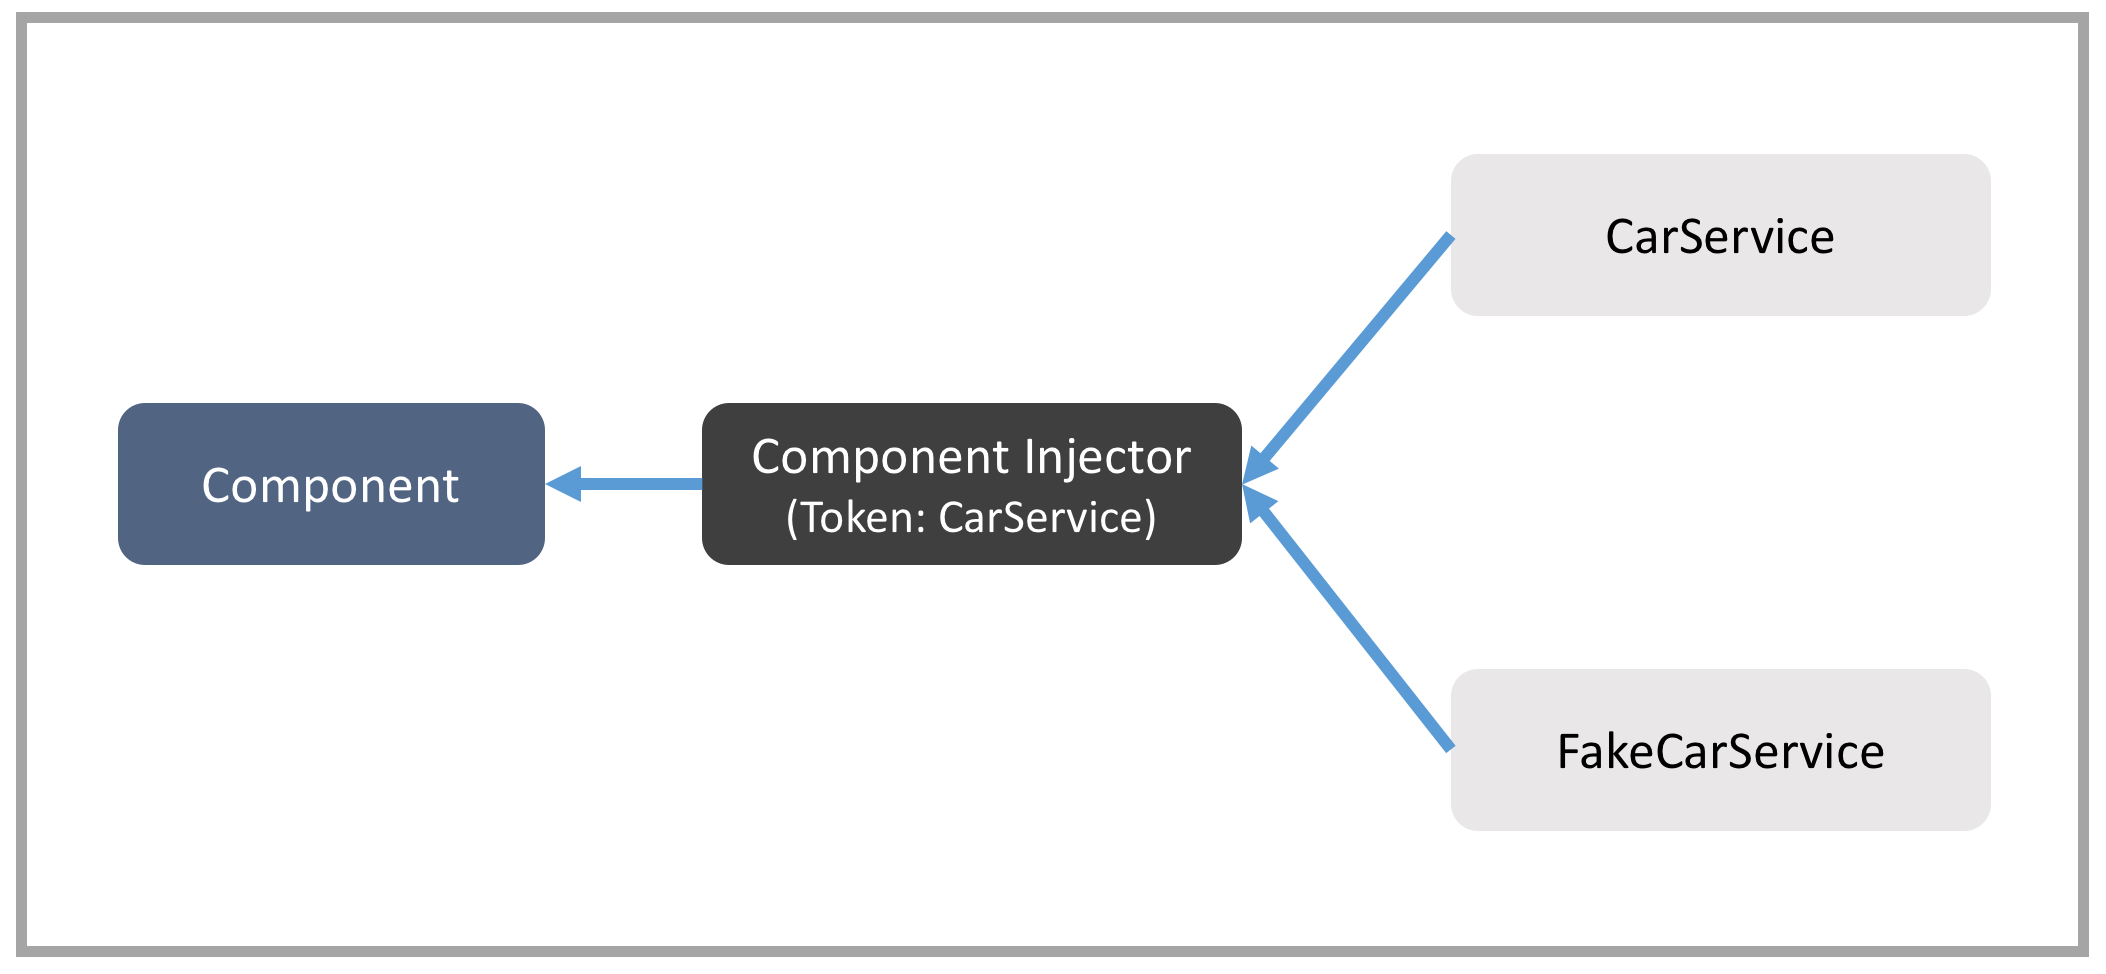
\includegraphics[width=0.8\linewidth]{kapitel3/component-injector.png}
 \caption{Component Injector \cite[343]{Angular2}}
 \label{service-injection}
\end{figure}
\vspace{0.3cm}

\ac{DI} wird in Angular über Provider konfiguriert.
Dies geschieht entweder auf Komponenten- oder Applikationsebene.
Wird ein Service über einen Provider im Bootstrap Prozess der Applikation referenziert,
so ist diese Instanz des Services in jede Komponente der Applikation injizierbar.
Wird der Provider erst in der Komponente definiert (Listing \ref{provider2}), so ist die Serviceinstanz nur in dieser Komponente sowie in
allen Kindkomponenten verfügbar. Desweiteren lassen sich Provider kombinieren, da diese überschreibbar sind.
Sollte also ein Serviceprovider auf Applikationsebene definiert sein (Listing \ref{provider1}), können dennoch weitere Provider innerhalb der Komponenten definiert werden.
Jedoch werden demnach auch mehrere Instanzen der Services erzeugt.
Es wäre also möglich, individuelle Singletons für bestimmte Komponentenbäume zu erzeugen \cite[286]{Angular2}.

\vspace{0.2cm}
\lstinputlisting[language=Javascript,label=provider1,caption=Provider im Bootstrap Prozess]{kapitel3/provider-example-root.ts}
\vspace{0.2cm}

\vspace{0.2cm}
\lstinputlisting[language=Javascript,label=provider2,caption=Provider in einer Komponente]{kapitel3/provider-example.ts}
\vspace{0.2cm}


\subsubsection{Services als Singletons}
\label{Services-als-Singletons}

Wie bereits erwähnt, ermöglichen \ac{DI} Provider, Services als Singleton zu instanziieren.
Dies bringt viele architektonische Vorteile mit sich. Services können auf der einen Seite genutzt werden,
um Funktionalität aus Komponenten zu abstrahieren, um in weiteren Komponeten verwendet zu werden.
Auf der anderen Seite können sie auch genutzt werden, um Daten multiplen Komponenten zur Verfügung zu stellen.
Das Angular Framework sorgt dafür, dass ein Service nur einmalig instanziiert wird. Daher erhalten alle
Komponenten, die den Service injizieren, dieselbe Referenz, somit dieselbe Instanz und daher dieselbe globale Datenbasis.
In einem Userservice könnte beispielweise eine Boolean Variable definiert sein, welche Auskunft darüber gibt,
ob ein User eingeloggt ist oder nicht \cite[308]{Angular2}.


\subsection{Data Binding}
Das in einer Komponente eingebundene Markup repräsentiert die Viewschicht einer Komponente.
Angular 2 besitzt zur Darstellung von Datenstrukturen eine komplexe, jedoch sehr ausdrucksstarke Template Syntax, siehe Listing \ref{ngtemplate}.
Variablen und Funktionen einer Komponente, können mit doppelt geschweiften Klammern in die View eingebunden werden.
Auf der Basis von HTML5 können zudem Schleifen und Fallunterscheidungen implementiert werden.
Der Gültigkeitsbereich des Templates bezieht sich, bezüglich Variablen und Funktionen, auf den Kontext der Komponente,
welche das Template in der Component Decoration referenziert \cite{Templ78:online}.

\vspace{0.3cm}
\lstinputlisting[language=HTML,label=ngtemplate,caption=Angular 2 Template Syntax]{kapitel3/template-example.html}

\subsection{Kommunikation}

Da eine Angular 2 Applikation ausschließlich aus Komponenten besteht, müssen diese zwangsweise miteinander
kommunizieren können. Für den Austausch von Daten gibt es verschiedene Ansätze.
Wie bereits in Sektion \ref{Services-als-Singletons} erwähnt, werden Services im Normalfall als Singleton
instanziiert und in Komponenten mittels \ac{DI} injiziert. Öffentliche Servicefunktionen können hier für den
Austausch von Daten genutzt werden. Über den synchronen Zugriff auf Variablen hinaus,
können Events in Komponenten oder Services definiert und ebenfalls abonniert werden,
um asynchrone Kommunikation applikationsintern zu ermöglichen. Die Auslagerung von Funktionalität in Services ergibt jedoch nur dann wirklich Sinn,
wenn diese auch als Singleton existieren kann.

Komponenten sind im Vergleich zu Services keine Singletons,
da sie mit jeder Verwendung in der Applikation neu instanziiert werden.
Variablen und Funktionen eingebundener Komponenten können durch die Annotationen \emph{@Input} und \emph{@Output}
direkt über ihren HTML Component Tag angesprochen werden. Im Normalfall werden bei der Instanziierung von Kindkomponenten
relevante Daten über den Input Tag übergeben und über den Output Kanal in Form von Event Emittern abonniert \cite{Angul94:online}.

Handelt es sich bei dem Kommunikationsziel speziell um Kindkomponenten und nicht um Nachbarkomponenten,
kann durch die Annotation \emph{@ViewChild} auf den öffentlichen Kontext der Kindkomponente zugegriffen werden.
Die Kommunikation geschieht in diesem Fall nicht über die View Layer der Komponenten,
sondern direkt von der Elternkomponente zu ihrer Kindinstanz \cite{ViewC61:online}.


\subsection{Change Detection}
\label{sec:change-detection}

Beim Start einer Angular2 Applikation wird nach anfänglichem Laden der Seite eine View gerendert.
Eine interne Datenstruktur wird dabei per Templating auf eine Viewstruktur, den DOM, abgebildet und dem Nutzer so mittels Text,
Formularen, Buttons, Bildern etc. visuell aufbereitet.
Gibt es nun Änderungen in der Datenstruktur zur Laufzeit, muss die View dementsprechend aktualisiert werden.
Zugriffe auf den DOM sind ressourcenintensiv, daher sollten DOM Manipulationen nicht inflationär stattfinden.
Datenänderungen können entweder durch User Events, XMLHttpRequests oder Timer (\emph{setTimeout}, \emph{setInterval}) ausgelöst werden.
Dies geschieht asynchron. Es ist also davon auszugehen, dass sobald eine asynchrone Aktivität innerhalb einer Komponente auftritt,
sich Daten geändert haben können und die View aktualisiert werden muss \cite{changedetection-explained}.

\subsection{NgZone}

Zones sind ein internes Feature der Programmiersprache Dart. Da Dart zu JavaScript compiliert werden kann,
können Zones ebenfalls in JavaScript genutzt werden. Zone.js ist als Portierung für JavaScript entstanden, welche in Angular2 genutzt wird.
Zones sind Ausführungskontexte (Scopes) für die Observation asynchroner Operationen.
Asynchrone Funktionen werden mittels \emph{Monkey Patching} überwacht und lösen innerhalb des entsprechenden Ausführungskontexts verschiedene Events aus.
NgZone ist ein Fork von zone.js, welcher die Basisfunktionalität um zusätzliche Events erweitert.
Relevant für die Change Detection ist dabei das event \emph{onTurnDone} \cite{changedetection-explained}.

\vspace{0.3cm}
``onTurnDone() - Notifies subscribers immediately after Angular’s zone is done processing the current turn and any micro tasks scheduled from that turn.''
\cite{ZONESINANGULAR2}
\vspace{0.3cm}

Sobald das \emph{onTurnDone} Event ausgelöst wird, löst NgZone wiederum einen \emph{tick} aus, welcher schlussendlich die Change Detection startet.
Jede Angular2 Komponente besitzt seinen eigenen Change Detector. Da eine Angular 2 Applikation aus einem Komponentenbaum besteht,
kann davon ausgegangen werden, dass sie ebenfalls aus einem Baum von Change Detektoren besteht, siehe Abbildung \ref{cdflow}.
Change Detection wird innerhalb dieses Baumes als unidirektionaler Datenfluss von oben nach unten, beginnend mit dem Rootknoten, ausgeführt.

Obwohl jede Komponente bei einem \emph{tick} auf Änderungen prüft, ist Angular 2 sehr schnell. Es können mehrere 100.000 Checks in wenigen Millisekunden durchgeführt werden,
da jede Komponente ihren eigenen Change Detector besitzt und es nicht eine große Instanz gibt, die alle Komponenten zeitgleich observieren muss.
Dies wird erreicht, indem Angular zur Laufzeit individuelle Change Detector Klassen für jede Komponente, entsprechend dem Datenmodell der Komponente, erzeugt.
Dieser Code kann von virtuellen Maschinen optimiert und daher vergleichsweise schnell ausgeführt werden \cite{changedetection-explained}.

\vspace{1cm}

\begin{figure}[ht]
 \centering
 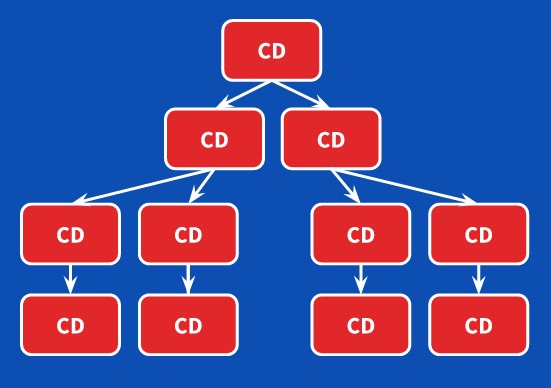
\includegraphics[width=0.7\linewidth]{kapitel3/cd-tree.jpg}
 \caption{Change Detection Flow \cite{changedetection-explained}}
\label{cdflow}
\end{figure}

\newpage
\section{Ionic}

Im nachfolgenden soll die Relevanz des Frameworks Ionic 2 bezüglich des Projekts \projectname{} evaluiert werden.

\subsection{Einführung}

Ionic 2 ist ein Open Source \ac{SDK} für die Entwicklung mobiler Applikationen auf Basis von Angular 2 und Cordova.
Auf Basis von Webtechnologien wie HTML5, CSS3 und JavaScript können Apps für iOS, Android und Windowsphone
entwickelt werden. Diese werden als hybride Apps bezeichnet,
da sie eine Mischform zwischen Web-Apps und nativen Applikationen darstellen.
Eine hybride App ist zunächst eine Webanwendung, die einen Browser für ihre Ausführung benötigt.
Als Browser wird die native Webview der jeweiligen Platform verwendet,
beispielsweise Safari für iOS und Chrome für Android.
Mithilfe von Cordova Plugins kann auf das \ac{API} des Systems zugegriffen werden,
um Funktionalitäten wie beispielsweise GPS, Telefonbuch und Kamera zu verwenden \cite{ionic34:online}.

\subsection{Ionic Components}

\ac{UI} Elemente einer Ionic Anwendung werden mithilfe von Angular 2 Komponenten realisiert.
Dabei können diese, wie in einer Angular 2 App, anhand ihres HTML Selektors wiederverwendet werden.
Komponenten können dabei wiederum verschachtelt werden, so dass ein Komponentenbaum entsteht.

Das Ionic \ac{SDK} stellt Entwicklern eine ganze Reihe an vorgefertigten Komponenten zur Verfügung,
welche native Standardelemente der jeweiligen Plattform abdecken. Beispiele dafür sind Buttons, Listen, Tabs oder ActionSheets.
Interessant dabei ist, dass die Optik der Komponente dabei dem \ac{CI} der Plattform entspricht \cite{ionic99:online}.

\subsection{Theming}
Theming wird in einer Ionic Anwendung durch \ac{CSS} realisiert.
Styles werden entweder in eine Komponente gekapselt oder global definiert.
Globale Stile können dabei plattformspezifisch oder plattformunabhängig definiert werden.
So befinden sich in einer klassischen Ionic 2 App individuelle Styles für iOS, Android und Windowsphone.
Dadurch kann das umzusetzende \ac{CI} flexibel getreu dem Standard der Plattform entwickelt werden.
Soll die Optik einer Anwendung für jede Plattform identisch sein,
können plattformunabhängige, globale Stile definiert werden \cite{ionic73:online}.


\subsection{Ionic Native}

Ionic Native ist ein Wrapper für Cordova Module in JavaScript und Typescript.
In der Vorgängerversion des \ac{SDK} wurden Cordova Plugins installiert und als globale Singletons registriert.
Beispielsweise war es möglich, aus jedem Kontext der Applikation heraus ``navigator.camera.getPicture(onSuccess, onFail)'' aufzurufen.
Ionic Native hingegen erlaubt Entwicklern, Module selektiv zu importieren, wodurch diverse Vorteile entstehen.
Globale Cordova Objekte werden vermieden, wodurch Code deutlich strukturierter und verständlicher wird.
Zudem werden Callbacks der Cordova Plugins mit Ionic Native in Promises oder Observables verpackt.
Dadurch entsteht ein einheitliches Interface im Stil von Angular 2 für die Nutzung dieser Module,
wodurch deren asynchrone Events bequemer observiert werden können.

Des Weiteren ist in Ionic Native eine Schicht für Fehlerbehandlung implementiert.
Ist ein Cordova Modul nicht installiert oder wird es falsch verwendet,
generiert Ionic Native Fehler und Warnungen, die für Entwickler unabdingbar sind.
In der Vorgängerversion des Ionic \ac{SDK} konnten Fehler, die durch falsche Verwendung von
Cordova Modulen aufgetreten sind, meist nur durch Ausprobieren oder Debugging des nativen Codes identifiziert werden
\cite{ionic55:online}.
Listing \ref{ionicnative} zeigt eine beispielhafte Implementierung der Kamera und GPS Schnittstellen durch Ionic-Native.

\vspace{0.3cm}
\lstinputlisting[language=JavaScript,label=ionicnative,caption=Ionic Native Beispiel \cite{ionic55:online}]{kapitel3/ionic-native-example.ts}


\subsection{Ökosystem Ionic}

``More than code. Ionic is an ecosystem. You'll find a suite of mobile development tools and resources at your disposal that make
Ionic the complete mobile dev package. It's the best way to build apps.'' \cite{Ionic20:online}
\vspace{0.3cm}

\paragraph{Ionic \ac{CLI}}
Die Ionic \ac{CLI} vereinfacht den Umgang mit Ionic Projekten erheblich. Zunächst können individuelle
Startertemplates anhand diverser Parameter generiert werden.
Das Framework erzeugt dabei voll funktionstüchtige Applikationen, die den Einstieg in das Framework erleichtern sollen.
\emph{Sidemenu} und \emph{Tabmenu} sind Beispiele für Templates, welche in Typescript oder JavaScript generiert werden können.
Darüber hinaus lassen sich Applikationen über die \ac{CLI} auf den Zielplattformen compilieren und auf angeschlossenen Geräten ausführen.

\paragraph{Ionic Creator}
ist ein Prototyping Tool, mit welchem Oberflächen statt
mit HTML und CSS per Mausklick kreiert werden können.
Dabei stehen von Beginn an eine Vielzahl von vorgefertigten Ionic Komponenten wie Buttons,
Labels und Eingabefelder zur Verfügung.
Diese werden per Drag and Drop eingefügt und positioniert. Der Prototyp lässt sich jederzeit
als \ac{APK} oder \ac{IPA} für Dritte exportieren oder kann auf einem angeschlossenen Gerät gestartet werden.

\paragraph{Ionic Lab}
ist eine visuelle Oberfläche zur Bedienung der Ionic \ac{CLI}.
Buildvorgang, Testing und Deployment wird mithilfe der Desktop-App für Mac, Windows, und
Linux speziell in Teams deutlich vereinfacht \cite{Ionic75:online}.

\subsubsection{Ionic Platform}

Ionic Platform ist eine Cloud, sowie eine Sammlung von Diensten für die Entwicklung,
Veröffentlichung und Skalierung von mobilen Apps. Zum Beispiel bietet Ionic Platform einen zentralen Dienst für die Nutzerverwaltung innerhalb einer App.
Nutzer können sich dabei klassisch per Mail oder per Single Sign-on über
Facebook, Google und Twitter registrieren und sind damit in der Applikation authentifiziert.
Zudem können registrierte Nutzer zentral in einer Weboberfläche verwaltet und gegebenenfalls mit Push Nachrichten adressiert werden.
Diese können dabei an alle Nutzer, oder ein definiertes Segment gerichtet werden.
Hierzu ist kein Server mit implementiertem \ac{APN} oder \ac{GCM} System notwendig, das Push System von Ionic deckt diese
Funktionalität bereits vollständig ab.

Zusätzlich kann die Cloud für das zentrale Deployment aller Zielplatformen genutzt werden.
Interessant hierbei ist, dass iOS Apps generiert werden können, auch wenn
keine macOS Umgebung zur Verfügung steht, da der Buildprozess in der Ionic Cloud stattfindet.
Ein App-Update muss nicht zwingend über den Appstore der Plattform geschehen,
da Änderungen, die sich nur auf den Webinhalt der App (also HTML, CSS und JS) beziehen,
beim Appstart aus der Cloud geladen werden können.
Dies ermöglicht es, Apps in Echtzeit zu deployen und Appstore Review Zyklen zu vermeiden.


\section{Electron}
\subsection{Allgemein}

Durch die stetige Entwicklung von Webbrowsern und Apps für Mobilgeräte haben Desktop-Applikationen in den letzten Jahren immer mehr an Bedeutung verloren.
Dennoch bieten sie gegenüber Anwendungen, die nur in Browsern ausgeführt werden, einige Vorteile.
Desktop-Anwendungen befinden sich im Dock beziehungsweise im Startmenü des Betriebssystems oder sind womöglich im Autostart referenziert.
Dadurch wirken sie präsenter, sind schneller zu erreichen und können selbst im minimierten Zustand noch Code ausführen.
Sie werden nicht durch den Kontext des Browsers limitiert und können APIs der Betriebssysteme nutzen \cite{Build58:online}.

Electron ist ein Framework zur Entwicklung nativer Desktop-Anwendungen, ebenfalls basierend auf Webtechnologien.
Atom, Visual Studio Code, Whatsapp und Slack sind erfolgreiche Beispiele für Anwendungen, die mithilfe von Electron
entwickelt wurden.
Der Fokus soll bei der Entwicklung auf die eigentliche Geschäftslogik der Anwendung und nicht auf plattformspezifischen
``hard parts'' der nativen Desktop Entwicklung gerichtet werden \cite{Elect57:online}.

\vspace{0.3cm}
``If you can build a website, you can build a desktop app. Electron is a framework for creating native applications
with web technologies like JavaScript, HTML, and CSS. It takes care of the hard parts so you can focus on the core of
your application.''
\cite{Elect57:online}

\subsection{Funktionsweise}
\label{sec:functionsweise}


Wie in Abbildung \ref{fig:electronprozess} dargestellt, werden beim Start einer
Electron Anwendung verschiedenen Prozesskontexte gestartet.
Zunächst startet der Hauptprozess (main process), in welchem grundlegende Konfigurationen vorgenommen werden können.
Die Besonderheit dieses Kontextes ist die Verfügbarkeit von Node.js.
Mit Node.js erhält man Zugriff auf Schnittstellen des Betriebssystems um beispielsweise Dateien lesen oder schreiben zu können.
Ferner wäre es im Hauptprozess möglich einen HTTP oder Websocket Server zu starten.

Der Hauptprozess instanziiert den Kontext der Webview, in Abbildung \ref{fig:electronprozess} wird dieser als render process bezeichnet.
Dieser beinhaltet eine Browserumgebung, welcher die \ac{UI} der Anwendung in einem für den Nutzer sichtbaren Fenster darstellt.
Die Webinhalte werden dabei mit Chromium, der quellofenen Basis von Google Chrome, gerendert \cite{Build58:online}.

\begin{figure}[htbp]
 \centering
 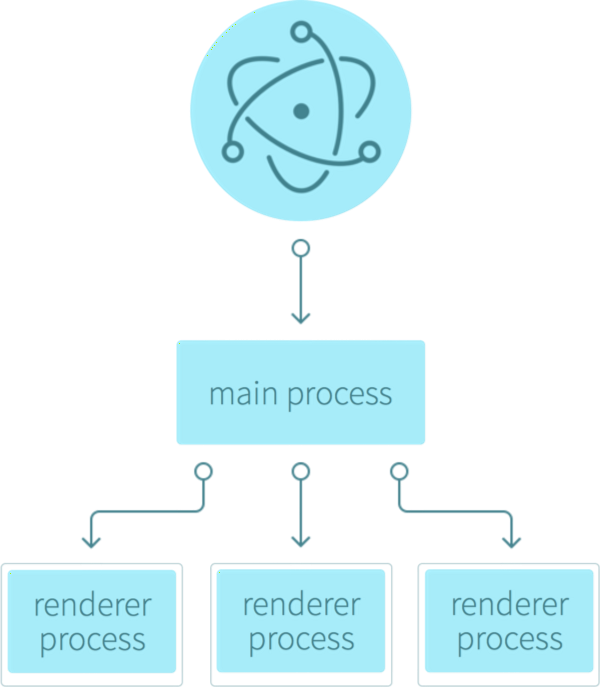
\includegraphics[width=0.4\linewidth]{kapitel3/electron-context.png}
 \caption{Electron Prozesse \cite{Build58:online}}
\label{fig:electronprozess}
\end{figure}


\subsection{Kommunikation}
\label{sec:Kommunikation}

Da Node.js nur im Hauptrozess von Electron genutzt werden kann, ist es erforderlich,
dass die verschiedenen Kontexte miteinander interagieren beziehungsweise kommunizieren können.
Dies kann, wie bereits in Sektion \ref{sec:functionsweise} angesprochen,
mithilfe eines lokalen API Servers oder Websockets stattfinden.
Die Electron API bietet eine weitere Möglichkeit für eine Interprozesskommunikation.
Dem main- und render Prozess wird jeweils eine IPC Event Emitter Instanz zur Verfügung gestellt,
über welche asynchrone Events gesendet und empfangen werden können.

\section{\ac{NPM}}

\ac{NPM} ist ein Package Manager für Node.js und JavaScript mit insgesamt mehr als 300.000 verschiedenen Paketen und
4.939.882.172 Paket Installationen im Juni 2016.
Open Source Pakete können kostenfrei veröffentlicht werden.
Für die Verwaltung von Closed Source Paketen wird ein Preismodell ab 7\$ pro Monat angeboten.
Dependencies des Projekts \projectname{}, also Pakete wie Angular, Ionic und Electron können vollständig
über \ac{NPM} geladen werden \cite{npm31:online}.

Ein \ac{NPM} Modul beinhaltet neben dem Programmcode eine Manifest Datei, in welcher relevante Metainformationen über das Modul selbst und den Autor gespeichert werden.
Zusätzlich können in dem Manifest (Package.json) post-Installation Scripte referenziert werden um
beispielsweise eine Transpilierung von TypeScript zu JavaScript vornzunehmen, nachdem das Modul als Abhängigkeit installiert wurde.
Die Veröffentlichtung in der Registry und damit auf \emph{npmjs.com} sowie der Updatevorgang eines Moduls geschieht über die \ac{CLI} von \ac{NPM}.

\section{Gulp}

Gulp ist ein Build System zur Ablaufoptimierung und Automatisierung komplexer Softwareprodukte.
Das System basiert auf Node.js Streams, kann jedoch auch für Plattformen wie Java, PHP und .Net verwendet werden.
Automatisierungen werden mit Gulp in Form von Tasks implementiert,
welche typischerweise Dateien lesen, diese innerhalb von Streams verarbeiten und das Ergebis wiederum auf die
Festplatte schreiben \cite{gulpj46:online}.
Tasks können dabei manuell, oder über Filewatcher durch Dateiänderungen ausgelöst werden.
Anwendungsfälle für Gulp Tasks sind beispielweise Transpilierung von Typescript zu JavaScript Code oder
Automatisierung von Deployment Prozessen. Die \ac{NPM} Registry beinhaltet bereits über 14.000 Open Source Plugins,
mit denen die Grundfunktinalität von Gulp erweitert werden kann \cite{resul14:online}.
Gulp selbst wurde im Juni 2016 2.304.745 mal per NPM installiert \cite{gulp17:online}.
